%Linea Para poder completar automaticamente las citas con el Sublime
%No hace el documento, se puede borrar esta linea si no se usa el Sublime
%------------------------------------------------------------------------------
 \newcommand{\NoBiblioEQ}[1]{
 \ifthenelse{\equal{#1}{verdadero}}{}{\bibliography{Referencias/base_bibliografica}}
 \NoBiblioEQ{verdadero}}
 %----------------------------------------------------------------------------- 

%Formato (Nombre de capitulo largo o corto), nombre del capitulo y estilo de la
%Portada del Capitulo
%------------------------------------------------------------------------------

 %Formato en si, titulo en un solo renglon
 \FormatoCapituloDosLineas
 
 %Nombre y etiquete para referir
 \chapter{Propiedades de transporte\index{transporte} de los sensores}
 \label{chap:Electroquimica}

 %Para que no salga el numero de pagina en la portada del capitulo
 \thispagestyle{empty}
	
 %Resumen del Capitulo en Italica
 \noindent\textit{Aca va todo el desarrollo de la fisicoquimica de los mesospororos, fenomenos de  transporte, adsorcion, lagmuir, propiedades de mediacion redox, catalisis, etc, etc.}

 %Indice de capitulo alineada al borde inferior de la pagina, nueva pagina
 \vfill
 \minitoc
 \newpage
 %-------------------------------------------------------------------------------

\section{Introducción}

	Una vez estudiados los distintos tratamientos de síntesis y realizada la fabricación de los sensores\index{sensor} se dedicará, en este capitulo, a estudiar las propiedades de los mismos para detectar y cuantificar una serie de sonda\index{sonda}s electroquímica\index{electroquimico}s\index{electroquimico} elegidas, precisamente, para poder evaluar distintos aspectos de transporte\index{transporte} a través de los sistemas nanoporosos. 
	Los sensores\index{sensor} están compuestos básicamente de una película delgada \index{película!delgada}de oro\index{oro} y una película delgada \index{película!delgada}nanoporosa\index{película!nanoporosa} de SiO$_2$. 

	La superficie\index{superficie} de las paredes dejan expuestos, hacia el interior de los poros, grupos silanoles los cuales pueden estar o no protonados.\cite{Brinker1990,Soler-Illia2011} 
			\begin{equation}
				\begin{aligned}
				\includegraphics[scale=0.75]{Esquemas/equilibriosilica.pdf}
				\label{eq:equilibriosilica}
				\end{aligned}
				\end{equation}
	La reacción \ref{eq:equilibriosilica} ejemplifica el equilibrio ácido-base que se establece en la superficie\index{superficie} de la sílice. El pKa del $\text{SiO}_2$ es menor a 4 y la mayoría de los autores coinciden en que el isoeléctrico (PI) varía de $1$ a $4$ dependiendo de  las distintas forma alotrópicas del óxido de silicio\index{silicio!oxido de}, en particular para el SiO$_2$ sintetizado vía sol-gel\index{sol-gel} el $\text{PI}\approx 2$ \cite{Kosmulski2002,Kosmulski2014,Schwarz1984,Si-HanWu2013}.
	Wu\index{Wu} y colaboradores\cite{Si-HanWu2013} analizaron, por un lado, el estado de carga superficial de nanoparticula\index{nanoparticula}s\index{nanoparticula} de sílice mesoporosa\index{película!mesoporosa} y, por otro, la tasa de condensación\index{condensación}. El gráfico de la figura \ref{fig:silica_ph} muestra como varían las razones  $\text{SiO}^{-}/\text{SiOH}$ y $\text{SiOH}_2^{+}/\text{SiOH}$ en función del pH\index{pH}; se puede apreciar que solo por encima de $\text{pH}\geq7$ se obtiene una superficie\index{superficie} de carga negativa donde todos los silanoles reaccionaron, cediendo su $\text{H}^{+}$, para convertirse en iones silanoatos; mientras que para pH\index{pH} bajos ($\text{pH}\leq1$), la sílice se vuelve inestable antes de llegar a un estado de carga completamente positivo y, solo queda, parcialmente positiva. En el mismo trabajo\cite{Si-HanWu2013} también plantean que la tasa de condensación\index{condensación} decrece por encima de $\text{pH}\geq7.5$ debido a entra en una zona de inestabilidad donde el óxido se disuelve, catalizado por el medio básico.
			\begin{figure}[th!]
			\centering
 	       	\includegraphics[width=0.70\textwidth]{Graficos/Silica-PH-Stability.pdf}
	       		\caption[Tasa de condensación\index{condensación} y estado de carga superficial]{Tasa de condensación\index{condensación} y estado de carga superficial para nanoparticula\index{nanoparticula}s\index{nanoparticula} de sílice en función de pH\index{pH}. Gráfico extraído de \textit{Synthesis of mesoporous silica nanoparticles} Chem. Soc. Rev., 42(9):3862, 2013.\cite{Si-HanWu2013}}
	         	\label{fig:silica_ph}
	     		\end{figure}
			
	%Del equilibrio se desprende que al incrementar el pH\index{pH} por encima de $2$ la película presentará una carga neta negativa, y, consecuentemente al disminuir el pH\index{pH} por debajo de $2$ la película será neutra o levemente positiva. 
	De hecho, Iler\index{Iler}, en su libro \textit{<<The Chemistry of Silica>>}, explica que la tasa de disolución de la sílice en medio acuoso depende de muchos factores y, que además, salvando el tipo de sílice, el proceso de disolución requiere de un catalizador. Presenta un gráfico de la tasa de disolución en función del pH\index{pH} (figura \ref{fig:disolucion_ph}) y postula que la tasa de disolución depende de la forma alotropica de la sílice, mientras que para formas mas porosas como el SiO$_2$ amorfo la cinética de disolución es mas rápida, para otras como el cuarzo se hace mucho mas lenta; por último aclara que se trata de un proceso de despolimerización vía hidrólisis, y la solubilidad es la concentración de Si(OH)$_4$ cuando alcanza un estado estacionario en el equilibrio despolimerazación-polimerización.\cite{iler1979}. 

			\begin{figure}[th!]
			\centering
 	       	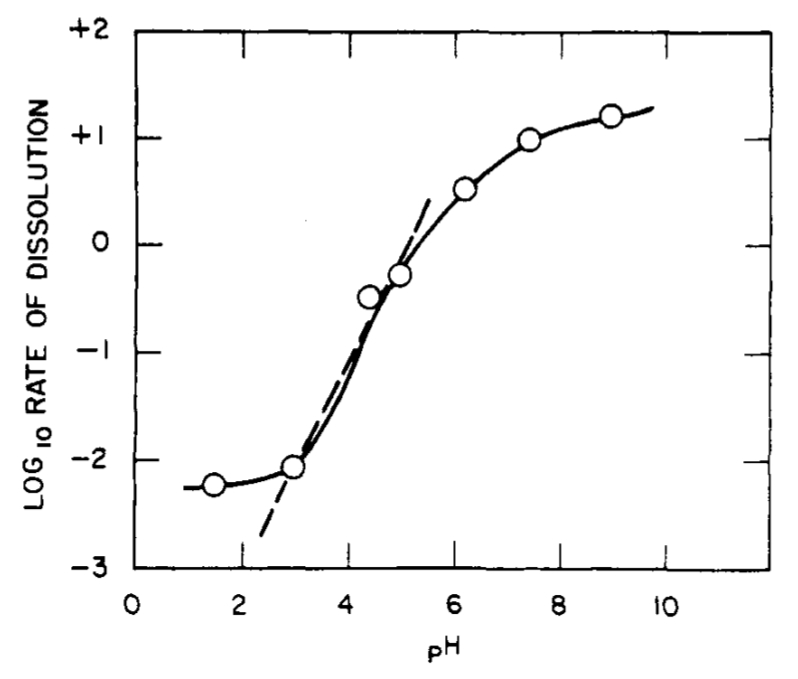
\includegraphics[width=0.70\textwidth]{Graficos/disolucion_ph.pdf}
	       		\caption[Tasa de disolución sílice en función del pH\index{pH}]{Tasa de disolución de la sílice en función de pH\index{pH}. Gráfico extraído de \textit{The chemistry of silica} Wiley 1ª edición, 1979.\cite{iler1979}}
	         	\label{fig:disolucion_ph}
	     		\end{figure}
	
	También propone un mecanismo en medio ácido\index{acido@ácido} catalizado por iones F$^-$, mientras que en medio básico\index{básico} el mecanismo es catalizado por iones OH$^-$, según el siguiente mecanismo:
			\begin{equation}
				\begin{aligned}
				\includegraphics[scale=0.60]{Esquemas/disolucionsilica.pdf}
				\label{eq:disolucionsilica}
				\end{aligned}
				\end{equation} 
	
	El mecanismo de \ref{eq:disolucionsilica} no está completamente consensuado en la literatura especializada, sin embargo todos los autores coinciden en que el óxido se vuelve inestable en cualquiera de sus forma alotrópicas a partir de un $\text{pH}\geq7$ y que se disuelve rápidamente para $\text{pH}\geq10$\cite{Kosmulski2002,Kosmulski2014,Schwarz1984,Si-HanWu2013,iler1979}.

	%Dependencia de la constante de K con el PH.... poner aqui el grafico, ecuacion y grafico de Wu2013 donde propone estado de carga y donde se muestra que recien a PH=5 se llega a un estado de carga copmpeltamente negativo.
	
				
	%ca tengo que poner como es la reaccion del punto isoeléctrico\index{punto isoeléctrico} del Sio2 o del punto de carga zero... o del pka??? Y tambien tengo que poner los antecendente de calvo, calvo y el otro del 2005. Y tambien entonces que la diferencia es el Au\index{oro} miniaturizacion, etc, etc mayores velocidades... etc. 
	%No olvidarse de los ferrocenos a distintas velociades de barrido

\section{Transporte de sonda\index{sonda}s: exclusión, permeación y preconcentración}

	Durante las próximas secciones se interpretarán los resultados obtenidos al colocar soluciones con sonda\index{sonda}s electroquímica\index{electroquimico}s\index{electroquimico}, con diferentes cualidades, sobre los sensores. Al\index{aluminio} ser, la fabricación de los sensores, una parte estructural de este trabajo, cabe aclarar sobre que sistemas que se realizaron los resultados de los experimentos que mostraremos durante el desarrollo de este capitulo. Se utilizó, indistintamente, películas de Au\index{oro} sobre sustratos varios (silicio, vidrio, flexible), con diseño ya transferido o sin transferir. Salvo que se aclare lo contrario, se trabajó siempre con sistemas con la película delgada \index{película!delgada}mesoporosa estrucutras con Pluronic F127\index{Pluronic F127} y sintetizada con el método de alto vacio\index{alto@alto vacío} (consultar sección \ref{sec:trat-vacio}, pág. \pageref{sec:trat-vacio}) ; todas las medidas fueron normalizadas por el área geométrica, de forma de facilitar la comparación cuando se trata de sensores\index{sensor} con distinto diseño; todas las medidas fueron llevadas a cabo a $\text{pH}\approx5,5$ en solución de KCl \SI{100}{\milli\Molar}, elegido con el propósito de tener una fuerte carga neta negativa dentro de la películas, y a su vez, no estar tan comprometido con la cinética de disolución de la sílice.

	\subsection{Caso 1: sonda\index{sonda} de carga negativa}

	El voltagrama de la figura \ref{fig:exclusion_vs_Au} muestra la respuesta de los sensores\index{sensor} cuando se colocan en una solución con una sonda\index{sonda} negativa. Como sonda\index{sonda} de carga negativa se utilizó ferro/ferriciunuro de potasio (\ferroferri, \SI{1}{\milli\Molar}) en proporciones equimolares. El voltagrama rojo corresponde a la respuesta en un electrodo de Au\index{electrodo!de Au}\index{oro} desnudo, mientras que la verde a un electrodo recubierto de \pdm.
	
			\begin{figure}[ht]
				\centering
		 	    \includegraphics[width=0.70\textwidth]{Graficos/ExclusionFcCN.pdf}
		        \caption[Exclusión electrostática]{Respuesta compartiva de un electrodo de Au\index{electrodo!de Au}\index{oro} recubierto con \pdmF\space y sin recubrir frente a una sonda\index{sonda} \ferroferri \SI{1}{\milli\Molar} en \SI{0.1}{\Molar} de KCl contra ESC.}
		        \label{fig:exclusion_vs_Au}
		      	\end{figure}
	
	 Al\index{aluminio} ser la sonda\index{sonda} de carga negativa, no es capaz de ingresar a la película (la cual está cargada negativamente), y, por lo tanto tampoco puede difundir hacia el electrodo, eso se refleja en el voltagrama donde no se observa ni reducción ni oxidación de la sonda\index{sonda}. La repulsión se debe a un efecto de exclusión electrostática. Este fenómeno de exclusión ya fue reportado por varios autores\cite{alberti2015,schmuhl2005,Andrieu-Brunsen2015,brunsen2011}. Al\index{aluminio} pH\index{pH} de trabajo, $\text{pH}=5,5$, los silinanoles están como silanolatos, como ya se explicó anteriormente, estableciendo una carga negativa en todo el espesor de la película delgada \index{película!delgada}de óxido.

	 Desde el punto del estudio de fenómenos de  transporte\index{transporte} esta sonda\index{sonda} no es especialmente útil, porque, como ya se demostró, no puede ingresar en la \pdm. Sin embargo, nos ofrece información importante sobre la integridad estructural de las películas delgadas, dicho de otro modo, al no obtener señal electroquímica\index{electroquimico} significa que, la sonda\index{sonda} no percola a través de la \pdm\space, que la \pdm\space se encuentra sin fisuras, agujeros o rajaduras y que recubre por completo el área del electrodo.

	 Por ende fue muy importante para corroborar (si no hay señal la película esta intacta, si hay señal esta el Au\index{oro} expuesto) el estado de las \pdm\space al finalizar experimentos donde se dudaba del estado de la película, de esta forma se utilizó esta sonda\index{sonda} a modo de <<experimento control>>, realizando una voltametría\index{voltametría} cíclica para comprobar que las películas no tuviera sitios de percolación.

	\subsection{Caso 2: sonda\index{sonda} de carga neutra}

	Ferroceno y todos los datos de permeacion. Calcinado vs Bajas Tcd 

	\subsection{Caso 3: sonda\index{sonda} de carga positiva}

			\begin{figure}[ht]
				\centering
		 	    \includegraphics[width=0.70\textwidth]{Graficos/Ru10mM-ventana-preconcentracion.pdf}
		        \caption[asd]{asd}
		        \label{fig:asd}
		      	\end{figure}

			\begin{figure}[ht]
				\centering
		 	    \includegraphics[width=0.70\textwidth]{Graficos/Ru10mM-Resumen.pdf}
		        \caption[asd]{asd}
		        \label{fig:asd}
		      	\end{figure}
		    
			\begin{figure}[ht]
				\centering
		 	    \includegraphics[width=0.70\textwidth]{Graficos/Ru10mM.pdf}
		        \caption[asd]{asd}
		        \label{fig:asd}
		      	\end{figure}

		    \begin{figure}[ht]
				\centering
		 	    \includegraphics[width=0.70\textwidth]{Graficos/Langmuir.pdf}
		        \caption[asd]{asd}
		        \label{fig:asd}
		      	\end{figure} 	
		      	      	      	
	pre-concentracion

	Rutenio\\
	*) Como es el modelo, porque se adsorbe como se adsorbe en el tiempo, primera demostracion\\
	*) Catalisis de la disolucion por electroquimica, estabilidad en el tiempo, ventana de trabajo\\
	*) Experimentos de adsorcion donde se remueve la solucion de ru\\
	*) Todos los graficos de Q vs V y Lagmuir donde se demuestra la adsorcion por la forma de la isorterma 
	*) Comparacion peliculas polimericas\\
	*) Cinetica de la disolucion calcinado Vs bajas T

\section{Mediacion redox y catalisis y simulacion}

\section{Modelo propuesto}

\section{Conclusiones parciales}

% 	Aca Hay que poner los graficos de 1mM de Ru para INTI\index{INTI} baja T y CNEA\index{CNEA} calcinado donde se muestra y se pueden vislumbrar los dos mecanismos de transporte\index{transporte} de carga, el de libre y el Ru adsorbido.!!!!

% 	Agragar todo lo del ferroceno, lo catalisis con HQ y tambien la mediacion con ferro/ferri

% 	Tambien poner curva de Lagmuir y curvas donse se ve como se disuelve el electrodo! SIEMPRE con cualquier sonda\index{sonda}

% 	Aca poner el grafico de estabilidad en funcion del tiempo, explicar que onda que se disuelve pero solo cuando se le hace EQ, que solo aguanta 48 HS.... que no es despegado, etc, etc, que otros sistemas con ITO tambien demostraron los mismos resultados, y que los experimentos siempre terminamos con ferri/ferro para demostrar que la membrana esta intacta.

% 	Preconcentacion, comparacion con calcindado y bajas T
% 	\marginpar{Probar el Au-CTAB en Vacio y calcinado con aminorutenio\index{aminorutenio} para ver comportamiento del film, tengo dos muestras buenas que puede servir... la de calcinado es imposible, porque va a dar mal por el AU.}
	

% 	Hay que tener en cuenta aqui el tema de la respuesta Eq que solo son sitios activos los adsorbido y que puede que haya mas Rutenio adsorbido en realiadad. Es una cota inferior de la concentracion dentro de lo poros. Además esta el tema del area, trabajamos siempre con el area geometrica pero se sabe que esta no es el area del electrodo activa sino que es mas..... ambos efectos van en el mismo camino a favor de una mayor concentracion.

%Ventana de trabajo antes de la solubilidad de las peliculas, porque se disuelven, etc. etc.

% 		 		\indent Esta etapa del trabajo involucró la síntesis por sol-gel\index{sol-gel} de películas delgadas de óxido de silicio\index{silicio!oxido de}\index{silicio} mesoporoso. Los sensores\index{sensor} están compuestos por tres elementos estructurales, el sustrato\index{sustrato} (silicio, vidrio, polímeros), los electrodos de Au\index{electrodo!de Au} y sobre ellos la <<película activa>>. Esta última es la que se encargará de atribuirle propiedades diferenciales a cada electrodo de cada arreglo de sensores. Como se explico con anterioridad, se escogió oxido se silicio\index{silicio} entre otras cosas por su rica diversidad química, por ser transparente en el UV/VIS, por ser un óxido de uso frecuente en microelectrónica\index{microelectrónica} y por su bajo costo.

% 	\subsection{Películas delgadas de silica mesoporosa}

% 				\indent Las peliculas fueron depositas por <<spin coating>> 80uL, 4000RPM

% 	\subsection{Caractización}
% 	comparaciones con el ITO, porque usamos Au. adherencia.

% Aca va todo el chorro del Au, del cambio de target, etc, etc. Tabla con todos los experimentos hechos, cambio de agua de las soluciones, cambio de electrolito sporte, cambio de sustrato, sin capa adherente.
% Caracterización electroquímica\index{electroquimico}, problemas, difusión\index{difusión}, XPS\index{XPS}, etc. ademas de medicdas de ACV? CV? Au\index{oro} de la CNEA\index{CNEA}, etc. ademas de la resistencia a la trasferencia de electronico. curvas a mas achatadas.

% \subsection{Soluciones a los problemas de Incompatibilidad}

% Cambio en el tarjet de Au, aca van las medidas electroquimicas de Au\index{oro} sobre el target de la CNEA\index{CNEA} y el del INTI\index{INTI} calcinados

% Cambio por ITO, porque si porque no

% Cambio en el tratamiento termico de la sintesis de los mesoporosos a baja T

% Aca va el cambio de au vs tratamientos de bajas temperaturas y aplicable a nuevos sustratos y por supuesto mucho mas economico (por el Au).,